\documentclass[10pt,landscape]{article}
\usepackage{amssymb,amsmath,amsthm,amsfonts}
\usepackage{multicol,multirow}
\usepackage{calc}
\usepackage{ifthen}
\usepackage[landscape]{geometry}
\usepackage[colorlinks=true,citecolor=blue,linkcolor=blue]{hyperref}
\usepackage{hyperref}
\usepackage{setspace}
\usepackage[utf8x]{inputenc}
\usepackage[english,russian]{babel}
\usepackage[para]{footmisc}
\usepackage{xcolor}
\usepackage{pagecolor,lipsum}
\usepackage{esint}
\usepackage{nicefrac}
\usepackage{graphicx}
\graphicspath{ {.} }
\usepackage[scr=boondoxo]{mathalfa}
%scr = mathpi%

\pagecolor{yellow!30!}

\ifthenelse{\lengthtest { \paperwidth = 11in}}
    { \geometry{top=.5in,left=.5in,right=.5in,bottom=.5in} }
	{\ifthenelse{ \lengthtest{ \paperwidth = 297mm}}
		{\geometry{top=1cm,left=1cm,right=1cm,bottom=1cm} }
		{\geometry{top=1cm,left=1cm,right=1cm,bottom=1cm} }
	}
\pagestyle{empty}
\makeatletter
\renewcommand{\section}{\@startsection{section}{1}{0mm}%
                                {-1ex plus -.5ex minus -.2ex}%
                                {0.5ex plus .2ex}%x
                                {\normalfont\large\bfseries}}
\renewcommand{\subsection}{\@startsection{subsection}{2}{0mm}%
                                {-1ex plus -.5ex minus -.2ex}%
                                {0.5ex plus .2ex}%
                                {\normalfont\normalsize\bfseries}}
\renewcommand{\subsubsection}{\@startsection{subsubsection}{3}{0mm}%
                                {-1ex plus 0ex minus .5ex}%
                                {0.5ex plus .2ex}%
                                {\normalfont\small\bfseries}}
                                
\newcommand{\spc}{\hspace*{1em}}
\renewcommand{\thefootnote}{(\arabic{footnote})}

\makeatother
\setcounter{secnumdepth}{0}
\setlength{\parindent}{0pt}
\setlength{\parskip}{0pt plus 0.5ex}
\onehalfspacing
% -----------------------------------------------------------------------

\title{}

\begin{document}

% \everymath{\displaystyle}
\raggedright
\footnotesize
\begin{center}
     \Large{\textbf{A formula summary for physics}} \\
\end{center}
\begin{multicols*}{3}
\setlength{\premulticols}{1pt}
\setlength{\postmulticols}{1pt}
\setlength{\multicolsep}{1pt}
\setlength{\columnsep}{2pt}

\section{Classical mechanics}
\subsection{Kinetics}
velocity: $\mathbf{v}=\frac{d\mathbf{r}}{dt}=r'_x \mathbf{i}+r'_y \mathbf{j}+r'_z \mathbf{k}$
\newline
acceleration: $\mathbf{a}=\frac{d\mathbf{v}}{dt}=v'_x \mathbf{i}+v'_y \mathbf{j}+v'_z \mathbf{k}$
\newline
motion laws:
\newline
\spc$v=v_0 +at$
\newline
\spc$x-x_0=v_0 t+ \frac{1}{2}at^2$
\newline
\spc$v^2-v_0^2=2a(x-x_0)$
\newline
\spc$x-x_0=\frac{(v_0+v)t}{2}$
\newline
centripetal acceleration: $a=\frac{v^2}{r}=\frac{4\pi ^2 r}{T^2}=4\pi ^2 rf^2=\omega ^2r$
\newline
velocity in two frames: $\mathbf{v}_{\mathrm{PA}}=\mathbf{v}_{\mathrm{PB}}+\mathbf{v}_{\mathrm{BA}}$
\newline
same acceleration measured in all frames: $\mathbf{a}_{\mathrm{PA}}=\mathbf{a}_{\mathrm{PB}}$

\subsection{Kinetics 2}
Newton's second law: $\mathbf{F}_\mathrm{T}=m\mathbf{a}$
\newline
Newton's third law: $\mathbf{F}_{\textrm{A to B}}=-\mathbf{F}_{\textrm{B to A}}$
\newline
\newline
acceleration of simple pulley: $a=\frac{m_1-m_2}{m_1+m_2}g$
\newline
drag force (body in fluid): $D=\frac{1}{2}C\rho Av^2$
\newline
\spc terminal speed: $v=\sqrt{\frac{2mg}{C\rho A}}$
\footnote{$C$: drag coefficient, $A$: effective cross-sectional area, $\rho$: air density.}
\newline
work: $W=\int \mathbf{F}\cdot d\mathbf{s}=\int_{x_i}^{x_f}F_x dx+\int_{y_i}^{y_f}F_y dy+\int_{z_i}^{z_f}F_z dz$
\newline
Hooke's law: $\mathbf{F}=-k\mathbf{x}$
\newline
\spc work by spring: $W=\frac{1}{2}kx_i^2-\frac{1}{2}kx_f^2$
\newline
kinetic energy: $K=\frac{1}{2}mv^2$
\newline
work-kinetic energy theorem: $W=K_f-K_i=\frac{1}{2}mv_f^2-\frac{1}{2}mv_i^2$
\newline
power: $P=\frac{dW}{dt}=\mathbf{F}\cdot \mathbf{v}$

\subsection{Kinetics 3}
definition of change in potential energy: $\Delta U=-W$
\newline
change in mechanical energy: $\Delta K+\Delta U=0$
\newline
total mechanical energy: $E=U+K$ (isolated)
\newline \newline
U-x graph:
\newline
external force: $F(x)=-\frac{d}{dx}U(x)$
\newline
neutral equilibrium: $E=U$
\newline
unstable equilibrium: $U''< 0, U'=0$
\newline
stable equilibrium: $U''> 0, U'=0$
\newline \newline
total m.energy of block-spring system: $E=\frac{1}{2}kx^2+\frac{1}{2}mv^2$
\newline
total m.energy of particle-earth system: $E=mgy+\frac{1}{2}mv^2$
\newline
conservation of energy: $\Delta K+\Delta U+\Delta E_{\textrm{internal}}\left ( + \textrm{other forms} \right )=0$ (isolated)
\newline
external work done: $W=\Delta K+\Delta U+\Delta E_{\textrm{internal}}$
\newline
change in energy: $\Delta E=\Delta K+\Delta U$
\newline
loss in mechanical energy (friction): $\Delta E=-fd$
\newline
energy loss due to emitted light: $E_x-E_y=hf$

\subsection{System kinetics}
centre of mass: $\mathbf{r}_{\mathrm{CM}}=\frac{1}{M} \sum _i m_i \mathbf{r}_i$
\newline
\spc continuous: $\mathbf{r}_{\mathrm{CM}}= \frac{1}{M}\int\mathbf{r}\rho dV= \frac{1}{V}\int\mathbf{r}dV$
\newline
\spc relation: $dm=\rho dV$
\newline \newline
linear momentum: $\mathbf{p}=m\mathbf{v}$
\newline
\spc relation: $K=\frac{p^2}{2m}$
\newline
net force: $\mathbf{F}_\mathrm{T}=\frac{d\mathbf{p}}{dt}$
\newline
Newton's second law: $\sum \mathbf{F}_{\textrm{external}}=M\mathbf{a}_{\mathrm{CM}}=\frac{d\mathbf{P}}{dt}$
\newline
conservation of linear momentum: $\mathbf{P}=\textrm{constant}$
\newline
\newline
циолковский's rocket formula:\newline
$\mathbf{F}=(\mathbf{v}-\mathbf{u})\frac{dm}{dt}+m\frac{d\mathbf{v}}{dt}$ or $\frac{d}{dt}m\mathbf{v}=\mathbf{F}+\mathbf{u}\frac{dm}{dt}$
\newline
\spc $v$: rocket's velocity in earth, $u$: fuel's velocity in earth
\newline \newline
change in translational k. energy: $\Delta K_{\mathrm{CM}}=F_{\mathrm{ext}}d_{\mathrm{CM}}$
\newline
König's theorem: $K=K_{\textrm{related to CM}}+\frac{1}{2}mv_{\mathrm{CM}}^2$

\subsection{Collisions}
impulse: $\mathbf{J}=\Delta \mathbf{p}=\int \mathbf{F}dt$
\newline
\newline
elastic collision:
\newline
\spc $v_1'=\frac{m_1-m_2}{m_1+m_2}v_1+\frac{2m_2}{m_1+m_2}v_2$
\newline
\spc $v_2'=\frac{m_2-m_1}{m_1+m_2}v_2+\frac{2m_1}{m_1+m_2}v_1$
\newline
\spc $v_\mathrm{CM}=\frac{P}{m_1+m_2}$
\newline \newline
complete inelastic collision: $m_1v_1+m_2v_2=(m_1+m_2)V_{\mathrm{CM}}$

\subsection{Rotation}
angular position: $\theta =s/r$
\newline
angular velocity: $\omega =\frac{d\theta}{dt}$
\newline
angular acceleration: $\alpha =\frac{d\omega}{dt}$
\newline
motion laws:
\newline
\spc $\omega =\omega _0+\alpha t$
\newline
\spc $\theta =\omega _0t+\frac{1}{2}\alpha t^2$
\newline
\spc $\omega ^2-\omega _0^2=2\alpha \theta $
\newline
\spc $\theta =\frac{(\omega _0+\omega )t}{2}$
\newline
linear-angular relation: $s=\theta r$, $v=\omega r$
\newline
\spc tangent acceleration: $a_t=\alpha r$
\newline
\spc radial acceleration: $a_r=\frac{v^2}{r}=\omega ^2r$
\newline \newline
rotational inertia: $I=\sum _i m_i r_i^2$
\newline
\spc r.i. for continuous objects: $I=\int r^2dm$
\newline
total rotational inertia: $I_{\mathrm{whole}}=\sum _i I_i$ (all to one axis)
\newline
parallel-axis theorem: $I=I_{\mathrm{CM}}+Mh^2$
\newline
perpendicular-axis theorem: $I_P=I_x+I_y$ (no thickness)
\newline
rotational kinetic energy: $K=\frac{1}{2}I\omega ^2$
\newline
torque: $\boldsymbol{\tau } =\mathbf{r}\times \mathbf{F}$
\newline
Newton's second law: $\tau _\mathrm{T}=I\alpha $
\newline
work: $W=\int F_t rd\theta =\int \tau d\theta $
\newline
power: $P=\frac{dW }{dt}=\tau \omega $
\newline
work-kinetic energy theorem: $W=\Delta K=\frac{1}{2}I\omega _f^2-\frac{1}{2}I\omega _i^2$

\subsubsection{Rotational inertia}
hoop, central axis: $I=MR^2$
\newline
hoop, diameter: $I=\frac{1}{2}MR^2$
\newline
annular cylinder, central axis: $\frac{1}{2}M\left ( R_1^2+R_2^2 \right )$
\newline
annular cylinder, central diameter,$\frac{1}{4}M\left ( R_1^2+R_2^2 \right )$
\newline
solid cylinder/disk, central axis: $\frac{1}{2}MR^2$
\newline
solid cylinder/disk, central diameter: $I=\frac{1}{4}MR^2+\frac{1}{12}ML^2$
\newline
rod, centre of length: $I=\frac{1}{12}ML^2$
\newline
rod, one end: $I=\frac{1}{3}ML^2$
\newline
triangle, parallel to base $a$ (whose height is $h$, through CM): $I=\frac{1}{18}Mh^2$
\newline
solid sphere, diameter: $I=\frac{2}{5}MR^2$
\newline
spherical shell, diameter: $I=\frac{2}{3}MR^2$
\newline
slab, centre: $I=\frac{1}{12}M(a^2+b^2)$
\newline
slab, along edge $b$:$I=\frac{1}{3}Ma^2$ 

\subsection{Rolling}
CM displacement/distance rolled: $x_{\mathrm{CM}}=\theta R$, $v_{\mathrm{CM}}=\omega R$
\newline
kinetic energy: $K=K_{\mathrm{rot}}+K_{\mathrm{tra}}=\frac{1}{2}I_{\mathrm{CM}}\omega ^2+\frac{1}{2}mv_{\mathrm{CM}}^2$
\newline
accleration of ideal yoyo: $a=-g(\frac{1}{1+I/MR^2})$
\newline
angular momentum: $\boldsymbol{\ell}=\mathbf{r}\times \mathbf{p}=\mathbf{r}\times m\mathbf{v}$
\newline
\spc a.m. for rigid, fixed axis: $L=I\omega $
\newline
angular impulse: $\Delta \boldsymbol{L}=\int \boldsymbol{\tau }dt$
\newline
Newton's second law: $\boldsymbol{\tau }_\mathrm{T}=\frac{d\boldsymbol{L}}{dt}$
\newline
conservation of angular momentum: $\boldsymbol{L}=\textrm{constant}$
\newpage

\subsection{Elasticity}
static equilibrium: $\mathbf{P}=0,\boldsymbol{L}=0$
\newline
requirements of equilibrium: $\sum \mathbf{F}_{\mathrm{ext}}=0,\sum \boldsymbol{\tau }_{\mathrm{ext}}=0$
\newline
tensile stress: $\frac{F}{A}=E\frac{\Delta L}{L}$, $E$: Young's modulus
\newline
sheering stress: $\frac{F}{A}=G\frac{\Delta x}{L}$, $G$: sheer modulus
\newline
hydraulic compression: $p=B\frac{\Delta V}{V}$, $B$: Bulk modulus

\subsection{Oscillation}
simple harmonic motion ($F=-m\omega^2x$):
\newline
\spc$\omega =\frac{2\pi }{T}=2\pi f$
\newline
\spc$x(t)=x_m \mathrm{cos}(\omega t+\phi )$
\newline
\spc$v(t)=-\omega x_m \mathrm{sin}(\omega t+\phi )$
\newline
\spc$a(t)=-\omega ^2 \, x(t)$
\newline \newline
linear oscillator
\newline
\spc definition: $\frac{d^2x}{dt^2}+\omega ^2x=0$
\newline
\spc angular frequency: $\omega =\sqrt{\frac{k}{m}}$
\newline
\spc period: $T=2 \pi \sqrt{\frac{m}{k}}$
\newline
\spc potential energy: $U(t)=\frac{1}{2}kx_m^2\mathrm{cos}^2(\omega t+ \phi)$
\newline
\spc kinetic energy: $K(t)=\frac{1}{2}kx_m^2\mathrm{sin}^2(\omega t+ \phi)$
\newline
\spc total energy: $E=\frac{1}{2}kx_m^2$
\newline
\spc series spring: $\frac{1}{K}=\sum _j \frac{1}{k_j}$, two: $K=\frac{k_1k_2}{k_1+k_2}$
\newline
\spc parallel spring: $K=\sum _j k_j$
\newline \newline
simple pendulum
\newline
\spc period: $T=2 \pi \sqrt{\frac{L}{g}}$
\newline
\spc restoring force: $F\approx -(\frac{mg}{L})s$
\newline \newline
torsion pendulum
\newline
\spc period: $T=2 \pi \sqrt{\frac{I}{\kappa }}$
\newline
\spc restoring torque: $\tau =-\kappa \theta $
\newline \newline
physical pendulum
\newline
\spc period: $T=2 \pi \sqrt{\frac{I}{mgh}}$
\newline
\spc restoring torque: $\tau =-(mg\mathrm{sin}\theta )h$
\newline \newline
damped simple harmonic motion
\newline
\spc damping force: $F_d=-bv$, $b$: damping constant
\newline
\spc definition: $\frac{d^2x}{dt^2}+\frac{b}{m}\frac{dx}{dt}+\frac{k}{m}x=0$
\newline
\spc \spc displacement: $x(t)=x_me^{-bt/2m}\mathrm{cos}(\omega _dt+ \phi)$
\newline
\spc angular frequency: $\omega_d=\sqrt{\frac{k}{m}-\frac{b^2}{4m^2}}$
\newline
\spc total energy: $E(t)\approx \frac{1}{2}kx_m^2e^{-bt/m}$

\subsection{Gravitation}
Newton's law of gravitation: $F=\frac{GMm}{r^2}$
\newline
gravitational constant: $G=6.67\cdot 10^{-11}\textrm{N}\cdot \textrm{m}^2/\textrm{kg}^2$
\newline
\spc differential: $dF=\frac{Gm_1}{r^2}dm$
\newline
gravitational field: $g=\frac{GM}{r^2}$
\newline
gravitational potential energy: $U=\int_{\infty }^{r}\frac{GMm}{x^2}dx=-\frac{GMm}{r}$
\newline
\spc escape speed: $v=\sqrt{\frac{2GM}{r}}$
\newline
\newline
plane motion of point mass:
\newline
\spc $a_r=\ddot{r}-r\dot{\theta}^2,a_\theta=2\dot{r}\dot{\theta}+r\ddot{\theta}$
\newline \newline
orbits:
\newline
\spc path of planet: $r=\frac{p}{1+e\mathrm{cos}\theta }$
\newline
\spc \spc $p=\frac{L^2}{GMm^2}$, $e=\sqrt{1+\frac{2EL^2}{G^2M^2m^3}}$
\newline
\spc net angular momentum: $L=mr^2\dot{\theta }$
\newline
\spc net mechanical energy: $E=\frac{1}{2}m(\dot{r}^2+r^2\dot{\theta} ^2)-\frac{GMm}{r}=\frac{1}{2}m\dot{r}^2+(\frac{L^2}{2mr^2}-\frac{GMm}{r})$
\newline
total energy of satellite-earth ellipse system:
$E=-K=-\frac{GMm}{2r}$
\newline
\spc perihelion: $r_1=a-c$
\newline
\spc aphelion: $r_2=a+c$
\newline
\spc\spc $a=\frac{r_1+r_2}{2}=-\frac{GMm}{2E}$, $c=\frac{r_2-r_1}{2}$, \spc\spc $b=\sqrt{a^2-c^2}=\sqrt{r_1r_2}=\frac{L}{\sqrt{-2mE}}$
\newline
total energy of satellite-earth hyperbola system: $E=\frac{GMm}{2r}$
\newline
total energy of satellite-earth parabola system: $E=0$
\newline
law of periods: $\frac{T^2}{r^3}=\frac{4 \pi ^2}{GM}$

\subsection{Fluids}
pressure: $p=\frac{\Delta F}{\Delta A}$ (all direction)
\newline
pressure in liquid: $p=p_0+\rho gh$
\newline
Pascal's principle: $\Delta p_{\textrm{int}}=\Delta p_{\textrm{ext}}$
\newline
Archimede's principle: $F_{\textrm{buoyancy}}=G_{\textrm{displaced water}}$
\newline
equation of continuity:
\newline
\spc volume flow rate $R=Av=\textrm{constant}$
\newline
\spc mass flow rate $m=Av\rho =\textrm{constant}$
\newline
Bernoulli's equation: $p+\frac{1}{2}\rho v^2+\rho gy=\textrm{constant}$

\subsection{Transverse waves}
transverse displacement: $y(x,t)=y_m\mathrm{sin}(kx-\omega t)$
\newline
\spc angular wave number: $k=\frac{2\pi }{\lambda }$
\newline
\spc waver number: $\kappa =\frac{1}{\lambda }$
\newline
\spc angular frequancy: $\omega =\frac{2 \pi}{T}$
\newline
\spc frequency: $f=\frac{1}{T}=\frac{\omega }{2 \pi}$
\newline
\spc wave speed: $v=\frac{\omega }{k}=\lambda f$
\newline
\spc \spc material expression: $v=\sqrt{\frac{\tau \textrm{(tension)}}{\mu (\textrm{density of media})}}$
\newline
\spc transverse speed: $u=\frac{\partial y}{\partial t}$
\newline
\spc average power: $\overline{P}=\frac{1}{2}\mu v\omega ^2y_m^2$
\newline \newline \newline \newline
adding waves
\newline
\spc superposition: $y=y_1+y_2=y_m\sin (kx-\omega t+\phi)+y_m\sin (kx-\omega t)$
\newline
\spc new wave: $y=(2y_m\mathrm{cos}\frac{1}{2}\phi)\mathrm{sin}(kx-\omega t+\frac{1}{2}\phi)$
\newline
\spc new amplitude: $2y_m\mathrm{cos}\frac{1}{2}\phi$
\newline
\spc phase shift: $+\frac{1}{2}\phi$
\newline
\newline
standing waves
\newline
\spc superposition: $y=y_1+y_2=y_m \sin (kx-\omega t)+y_m \sin (kx+\omega t)$
\newline
\spc new wave: $y=[(2y_m)\mathrm{sin}kx]\mathrm{cos}\omega t$
\newline
\spc new amplitude: $2y_m\mathrm{sin}kx$
\newline
\spc nodes: $x=n\frac{\lambda }{2}, n=0,1,2,...$
\newline
\spc antinodes: $x=(n+\frac{1}{2})\frac{\lambda }{2}, n=0,1,2,...$
\newline
\spc resonant frequency: $f_r=\frac{v}{\lambda }=\frac{v}{2l}n, n=1,2,3,...$

\subsection{Longitudinal waves}
speed of sound: $v=\sqrt{\frac{B}{\rho }}$
\newline
\spc bulk modulus: $B=-\frac{\Delta p}{\Delta V/V}(=\rho v^2)$
\newline
longitudinal displacement: $s=s_m\mathrm{cos}(kx- \omega t)$
\newline
air pressure: $\Delta p=\Delta p_m\mathrm{sin}(kx-\omega t)$
\newline
\spc relation: $\Delta p_m=(v\rho \omega )s_m$
\newline
\newline
interference
\newline
\spc phase shift: $\phi=\frac{\Delta d}{\lambda }2\pi$
\newline
\spc fully constructive: $\phi=m2\pi, m=0,1,2,...$
\newline
\spc fully destructive: $\phi=(m+\frac{1}{2})2\pi, m=0,1,2,...$
\newline
\newline
sound intensity: $I=\frac{1}{2}\rho v\omega ^2s_m^2$
\newline
sound level: $\beta =(10\textrm{ dB})\mathrm{log}(\frac{I}{I_0})$
\newline
\spc standard reference intensity: $I_0=10^{-12}\textrm{W}/\textrm{m}^2$
\newline \newline
resonant frequency
\newline
\spc pipe, two opens: $f_r=\frac{v}{\lambda }=\frac{v}{2L}n,n=1,2,3$
\newline
\spc pipe, one open: $f_r=\frac{v}{\lambda }=\frac{v}{4L}n,n=1,3,5,...$
\newline
beat frequency: $f_{beat}=f_1-f_2$
\newline
\newline
doppler effect: $f'=f\frac{v\pm v_L}{v\mp v_S}$
\newline
cone angle at supersonic speed: $\mathrm{sin}\theta =\frac{v}{v_s}$
\newpage
\section{Heat, Second law of thermodynamics}

\subsection{Heat}
coefficient of linear expansion: $\alpha =\frac{\Delta L/L}{\Delta T}$
\newline
\spc area expansion: $\beta =2\alpha $
\newline
\spc volume expansion: $\gamma =3\alpha $
\newline
heat capacity: $Q=cm(T_f-T_i)=C(T_f-T_i)$
\newline
heat of transformation: $Q=Lm$
\newline
volume work: $W=\int_{V_i}^{V_f}pdV$
\newline

first law of thermodynamics: $\Delta E_\textrm{int}=E_{\textrm{int,f}}-E_{\textrm{int,i}}=Q-W$
\newline
rate of heat transfer: $H=\frac{Q}{t}=kA\frac{T_H-T_C}{L}$\footnote{$k$: media's thermal conductivity.}
\newline
\spc multiple slabs: $H=A\frac{T_H-T_C}{\sum (L/k)}$

\subsection{Kinetic theory of gases}
ideal gas law: $pV=nRT$
\newline 
gas constant $R=8.31\textrm{J}/\textrm{mol}\cdot \textrm{K}$
\newline
volume work of expansion at constant pressure: $W=\int \frac{nRT}{V}dV=nRT \, \mathrm{ln}(\frac{V_f}{V_i})$
\newline
gas pressure: $p=\frac{nMv_{\textrm{rms}}^2}{3V}$
\newline
translational kinetic energy: $\overline{K}=\frac{3}{2}kT$
\newline 
Boltzman constant $k=R/N_A$
\newline
mean free path: $\lambda =\frac{1}{\sqrt{2}\pi dN/V}$\footnote{$d$: diameter, $N$: number of molecules.}
\newline
Maxwell's speed distribution: $P(v)=4\pi (\frac{M}{2 \pi RT})^{3/2}v^2e^{-Mv^2/2RT}$
\newline
\spc most propable speed: $v_p=\sqrt{\frac{2RT}{M}}$
\newline
\spc average speed: $\overline{v}=\sqrt{\frac{8RT}{\pi M}}$
\newline
\spc rms speed: $v_{\mathrm{rms}}=\sqrt{\frac{3RT}{M}}$
\newline
internal energy of monoatomic gas: $E_{\mathrm{int}}=(nN_A)\overline{K}=\frac{3}{2}nRT$
\newline
\spc monoatom: 3/2 ($f=1$)
\newline 
\spc diatom: 5/2 ($f=2$)
\newline
\spc 5-atom: 3 ($f=5$)
\newline
molar specific heat of monoatomic gas at constant volume: $C_v=\frac{3}{2}R=12.5\,\textrm{J/molK}$
\newline
\spc constant volume, change in internal energy: 
\newline
\spc $\Delta E_{\textrm{int}}=Q=nC_v(T_f-T_i)$
\newline
molar specific heat of monoatomic gas at constant pressure: $C_p-C_v=R$
\newline
\spc heat: $Q=nC_p(T_f-T_i)$
\newline
\spc work: $W=nR(T_f-T_i)$
\newline
law of adiabatic expansion: $pV^\gamma =\textrm{constant}$, or $TV^{\gamma -1}=\textrm{constant}$
\newline
\spc $\gamma =C_p/C_v=1+2/f$

\subsection{Second law of thermodynamics}
thermal effiency of engine: $e=\frac{|W|}{|Q_H|}=\frac{|Q_H|-|Q_C|}{|Q_H|}$
\newline
\spc max: $e_{\mathrm{Car}}=\frac{T_H-T_C}{T_H}$
\newline
coefficient of performance of refrigerator: $e=\frac{|Q_C|}{|W|}=\frac{|Q_C|}{|Q_H|-|Q_C|}$
\newline
\spc max: $e_{\mathrm{Car}}=\frac{T_C}{T_H-T_C}$
\newline
first law of thermodynamics in closed system: $|W|=|Q_H|-|Q_C|$
\newline
entropy: $dS=\frac{dQ}{T}$ and $∮ dS\leq 0$
\newline
reversible process: $S_f-S_i=\int _i^f dS=\int _i^f \frac{dQ}{T}$
\newline
free expansion: $S_f-S_i=\frac{1}{T}\int _i^f dQ=nR \, \mathrm{ln}\frac{V_f}{V_i}$
\newline
irreversible heat transfer: $S_f-S_i=cm\, \mathrm{ln}\frac{T^2}{T^2-\Delta T^2}$

\section{Electricity and Magnetism}
\subsection{Electrostatic forces}
Coulomb's law: $F=\frac{1}{4 \pi \epsilon _0}\frac{q_1q_2}{r^2}$
\newline
permitivity constant in vacuum: $\epsilon_0=8.85\cdot 10^{-12}\,\textrm{C}^{2}/\textrm{N}\cdot \textrm{m}^{2}$
\newline
charge is quantized: $q=ne$
\newline
\spc elementary charge $e=1.6\cdot 10^{-14}\,\textrm{C}$
\subsubsection{Electric field}
electric field: $\mathbf{E}=\frac{\mathbf{F}}{q_0}$
\newline
\spc differential: $d\mathbf{E}=\frac{1}{4\pi \epsilon _0}\frac{dq}{r^3}\mathbf{r}$ ($r$ from $dq$ to point)
\newline
\spc point charge: $E=\frac{1}{4 \pi\epsilon _0}\frac{q}{r^2}$
\newline
\spc straight rod (perpendicular): $E=\frac{\lambda a}{2\pi \epsilon _0 r}\frac{1}{\sqrt{4r^2+a^2}}$
\newline
\spc arc (to centre): $E=\frac{\lambda }{4 \pi \epsilon _0r}(2\mathrm{sin}\frac{\theta }{2})$
\newline
\spc ring (perpendicular): $E=\frac{qz}{4 \pi \epsilon _0(z^2+R^2)^{3/2}}$
\newline
\spc round disk (perpendicular): $E=\frac{\sigma }{2 \epsilon _0}(1-\frac{z}{\sqrt{z^2+R^2}})$
\newline
electrostatic force in a field: $\mathbf{F}=q\mathbf{E}$ (signed)
\subsubsection{Gauss' law}
Gauss' law: $\Phi _E=\oiint \mathbf{E}\cdot d\mathbf{S}=\frac{q}{\epsilon _0}$
\newline
\spc conducting surface: $E=\frac{\sigma }{\epsilon _0}$
\newline
\spc nonconducting surface: $E=\frac{\sigma }{2\epsilon _0}$
\newline
\spc straight rod: $\frac{\lambda }{2\pi r\epsilon _0}$
\newline
\spc two conducting plates (+ greater): $|E_L|=|E_R|=|E_{(+)}-E_{(-)}|$, $|E_{\textrm{in}}|=E_{(+)}+E_{(-)}=\frac{\sigma _1+\sigma _2}{\epsilon _0}$
\newline
\spc shell: $E=\frac{1}{4\pi \epsilon _0}\frac{q}{r^2}$ (outside), $E=0$ (inside)
\newline
\spc sphere: $E=\frac{1}{4\pi \epsilon _0}\frac{q}{r^2}$ (outside), $E=\left ( \frac{q}{4\pi \epsilon _0R^3} \right )r$ (inside)
\newline
\spc cylinder: $E=\frac{R^2\rho }{2\epsilon _0r}$ (outside), $E=\frac{\rho }{2\epsilon _0}r$ (inside)
\subsubsection{Potential}
work: $W=\int \mathbf{F}\cdot d\mathbf{s}=q_0\int \mathbf{E}\cdot d\mathbf{s}$
\newline
electric potential difference: $\Delta V=-\frac{W_{if}}{q_0}=\frac{\Delta U}{q_0}$
\newline
E-V relation: $\mathbf{E}=-\nabla V$, $V=-\int _{i_0}^f \mathbf{E}\cdot d\mathbf{s}$
\newline
electric field of parallel plates: $E=\frac{\Delta V}{\Delta d}$
\newline
point charge: $V=\frac{1}{4\pi \epsilon _0}\frac{q}{r}$(signed)
\newline
\spc discrete points: $V=\frac{1}{4\pi \epsilon _0}\sum _i\frac{q_i}{r_i}$
\newline
\spc continuous charge: $V=\frac{1}{4\pi \epsilon _0}\int \frac{dq}{r}$
\newline
\spc rod (perpendicular to one end): $V=\frac{\lambda }{4\pi \epsilon _0}\, \mathrm{ln}(\frac{L+(L^2+d^2)^{1/2}}{d})$
\newline
\spc arc (to centre): $V=\frac{\lambda \theta }{4\pi \epsilon _0}$
\newline
\spc ring (perpendicular): $V=\frac{q}{4\pi \epsilon_0\sqrt{z^2+R^2}}$
\newline
\spc disk (perpendicular): $V=\frac{\sigma }{2\epsilon _0}(\sqrt{z^2+R^2}-z)$

\subsection{Current and circuits}
current: $i=\frac{dq}{dt}$
\newline
current density: $J=i/A$
\newline
\spc relation: $i=\iint \mathbf{J}\cdot d\mathbf{A}$
\newline
\spc draft speed: $\mathbf{v}_\mathrm{d}=\mathbf{J}/(ne)$\footnote{ $n$: number of carriers per unit volume.}
\newline
resistance law: $R=\frac{V}{i}$
\newline
isotropic resistivity: $\rho=E/J$
\newline
\spc relation: $\mathbf{E}=\rho \mathbf{J}$
\newline
conductivity: $\sigma =1/\rho $
\newline
resistance: $R=\rho \frac{L}{A}$
\newline
\spc variation with temperature: $\rho -\rho _0=\rho _0\alpha (T-T_0)$\footnote{$\rho$: temperature coefficient of resistivity.}
\newline
\spc \spc$T_0=293\,\textrm{K}$, $\rho_0=1.69\,\mu\Omega\cdot\textrm{cm}$
\newline
rate of electricity supply: $P=iV$
\newline
\spc resistive dissipation: $P=i^2R=\frac{V^2}{R}$
\newline
electromotive force: $\mathscr{E} =\frac{dW}{dq}$
\newline
\spc supplying current: $i=\frac{\mathscr{E} }{R}$
\newline \newline
Kirchhoff's circuit laws
\newline
\spc resistance rule: $\Delta V=-iR$ (current), $\Delta V=+iR$ (opposite)
\newline
\spc emf rule: $\Delta V=+\mathscr{E} $ (current), $\Delta V=-\mathscr{E} $ (opposite)
\newline \newline
series charge: $q=q_1=q_2=...$
\newline
parallel charge: $q=\sum_j q_j$
\newline
series current: $i=i_1=i_2=...$
\newline
parallel current: $i=\sum_j i_j$
\newline
series voltage: $V=\sum _j V_j$
\newline
parallel voltage: $V=V_1=V_2=...$
\newline
series resistance: $R=\sum _j R_j$
\newline
parallel resistance: $\frac{1}{R}=\sum _j \frac{1}{R_j}$, two: $R=\frac{R_1R_2}{R_1+R_2}$
\newpage

\subsection{Capacitance}
capacitance: $C=\frac{q}{V}$
\newline
\spc parallel-plate: $C=\epsilon _0\frac{A}{d}$
\newline
\spc cylindrical: $C=2\pi \epsilon _0L\frac{1}{\mathrm{ln(b/a)}}$
\newline
\spc spherical: $C=4\pi \epsilon _0\frac{ab}{b-a}$
\newline
\spc isolated sphere: $C=4\pi \epsilon _0R$
\newline
series capacitor: $\frac{1}{C}=\sum_{j}\frac{1}{C_j}$
\newline
parallel capacitor: $C=\sum _j C_j$
\newline
work to charge capacitor: $W=\int dW=\int V'dq'$
\newline
\spc potential energy: $U=\frac{\epsilon_0AV^2}{2d}$
\newline
potential energy(parallel-plate): $U=\frac{q^2}{2C}=\frac{1}{2}CV^2$
\newline
volume energy density: $u=\frac{1}{2}\epsilon _0E^2$
\newline
\spc $q$ unchanged: $U_f=U_i/\kappa $
\newline
\spc $V$ unchanged: $U_f=\kappa U_i$
\newline \newline
RC circuit
\newline
\spc charging equation: $R\frac{dq}{dt}+\frac{q}{C}=\mathscr{E} $
\newline
\spc \spc charge function: $q=C\mathscr{E} (1-e^{-t/\tau _C })$
\newline
\spc \spc current function: $i=(\frac{\mathscr{E} }{R})e^{-t/\tau _C }$
\newline
\spc discharging equation: $R\frac{dq}{dt}+\frac{q}{C}=0 $
\newline
\spc \spc charge function: $q=q_0e^{-t/\tau _C }$
\newline
\spc \spc current function: $i=-i_0e^{-t/\tau _C }$
\newline
\spc capacitive time constant $\tau _C=RC$

\subsection{Magnetism}
force due to moving charge: $\mathbf{F}_B=q\mathbf{v}\times \mathbf{B}$
\newline
force due to current-carrying wire: $\mathbf{F}_B=i\mathbf{L}\times \mathbf{B}$ \newline
\spc $L$ along direction of conventional $i$
\newline
circular motion under $F_B$: $qvB=m\frac{v^2}{r}$
\newline
\spc period: $T=\frac{2\pi m}{qB}$
\newline
Hall effect, density of carriers: $n=\frac{Bi}{Vle}$
\newline
\spc $l=A/d$: thinkness of strip
\newline
Biot-Savart law: $d\mathbf{B}=\frac{\mu _0}{4\pi }\frac{id\mathbf{s\times \mathbf{r}}}{r^3}$
\newline
vacuum permeability: $\mu_0=4\pi\cdot10^{-7}\textrm{T}\cdot \textrm{m}/\textrm{A}$ (H/m)
\newline
\spc point charge: $B=\frac{\mu_0}{4\pi}\frac{qv}{r^2}$
\newline
\spc arc (to centre): $B=\frac{\mu _0i\theta }{4\pi R}$
\newline \newline
Ampere's circuital law: $\oint \mathbf{B}\cdot d\mathbf{s}=\mu _0i$
\newline
\spc long straight wire: $B=\frac{\mu _0i}{2\pi r}$
\newline
\spc solid wire: $B=\frac{\mu _0i}{2\pi r}$ (outside), $B=(\frac{\mu _0i}{2\pi R^2})r$ (inside)
\newline
\spc ideal solenoid: $B=\mu _0i_0n$, $n=N/L$: turns per unit length
\newline
\spc ideal toroid: $B=\frac{\mu _0i_0N}{2\pi r}$
\newline \newline
induced emf: $\mathscr{E} =-\frac{d\Phi _B}{dt}=-\frac{d}{dt} \iint \mathbf{B} \cdot d\mathbf{S}$
\newline
\spc for coils: $\mathscr{E} =-N\frac{d\Phi _B}{dt}$
\newline
Maxwell-Faraday equation: $\oint \mathbf{E}\cdot d\mathbf{s}=-\frac{d}{dt} \iint \mathbf{B}\cdot d\mathbf{S}$
\newline
\spc induced electrodynamic field, circle:
\\\spc$E=\frac{R^2}{2}\frac{dB}{dt}\frac{1}{r}$ (outside), $E=\frac{1}{2}\frac{dB}{dt}r$ (inside)

\subsection{Inductance}
inductance: $L=\frac{N\Phi _B}{i}$
\newline
\spc solenoid: $L/l=\mu _0n^2A$
\newline
\spc toroid: $L=\frac{\mu _0N^2h}{2\pi} \, \mathrm{ln}(\frac{b}{a})$
\newline
self-induced emf: $\mathscr{E} _L=-L\frac{di}{dt}$
\newline
potential energy: $U_B=\frac{1}{2}Li^2$
\newline
energy density: $u_B=\frac{B^2}{2\mu _0}$
\newline \newline
LR circuit
\newline
\spc rise in current: $iR+L\frac{di}{dt}=\mathscr{E} $
\newline
\spc\spc current function: $i=\frac{\mathscr{E} }{R}(1-e^{-t/\tau _L})$
\newline
\spc decay in current: $iR+L\frac{di}{dt}=0$
\newline
\spc\spc current function: $i=i_0e^{-t/\tau _L}$
\newline
\spc inductive time constant: $\tau _L=L/R$
\newline \newline
series inductance: $L=\sum _j L_j$
\newline
parallel inductance: $\frac{1}{L}=\sum _j \frac{1}{L_j}$
\newline
mutual induction, two coils: 
\newline
\spc $\mathscr{E} _2=-M\frac{di_1}{dt}$, $\mathscr{E} _1=-M\frac{di_2}{dt}$
\newline \newline
LC oscillation
\newline
\spc definition: $\frac{d^2q}{dt^2}+\frac{1}{LC}q=0$
\newline
\spc\spc charge function: $q=Q\mathrm{cos}(\omega t+\phi)$
\newline
\spc angular frequency: $\omega =\frac{1}{\sqrt{LC}}$
\newline
\spc electric potential energy: $U_E=\frac{Q^2}{2C}\mathrm{cos}^2(\omega t+\phi)$
\newline
\spc magnetic potential energy: $U_B=\frac{Q^2}{2C}\mathrm{sin}^2(\omega t+\phi)$
\newline
\spc total energy: $U=\frac{Q^2}{2C}$
\newline \newline
series RLC oscillation
\newline
\spc net energy dissipation: $\frac{dU}{dt}=-i^2R$
\newline
\spc definition: $\frac{d^2q}{dt^2}+\frac{1}{LR}\frac{dq}{dt}+\frac{1}{LC}q=0$
\newline
\spc \spc charge function: $q=Qe^{Rt/2L}\mathrm{cos}(\omega 't+\phi)$
\newline
\spc angular frequency: $\omega '=\sqrt{\omega ^2-(R/2L)^2}$

\subsection{Electromagnetic waves}
magnetic field induced by electric field: $\oint \mathbf{B}_E\cdot d\mathbf{s}=+\mu _0\epsilon _0\frac{d\Phi _E}{dt}=+\mu _0\epsilon _0\frac{d}{dt}\iint\mathbf{E}\cdot d\mathbf{S}$
\newline
"displacement current" between parallel plates, circle: 
\newline
\spc $B=\frac{\mu _0\epsilon _0R^2}{2}\frac{dE}{dt}\frac{1}{r}$ (outside), $\frac{\mu _0\epsilon _0}{2}\frac{dE}{dt}r$ (inside)
\newline
displacement current: $i_d=\epsilon _0\frac{d\Phi _E}{dt}$
\newline \newline 
Electromagnetic waves
\newline
\spc B and E are in phase:
\newline
\spc\spc $E=E_m\mathrm{sin}(kx-\omega t)$
\newline
\spc\spc $B=B_m\mathrm{sin}(kx-\omega t)$
\newline
\spc wave speed: $c=\frac{\omega }{k}$
\newline
\spc magnitude ratio: $\frac{E_m}{B_m}=c$
\newline
\spc speed of light: $c=\frac{1}{\sqrt{\epsilon _0\mu _0}}$
\newline
\spc direction of wave/poynting vector: $\mathbf{S}=\frac{1}{\mu _0}\mathbf{E}\times \mathbf{B}$
\newline \newline
plane wave's instantaneous flow rate: $S=\frac{1}{c\mu _0}E^2$ ($S=P/A$)
\newline
wave intensity: $I=\overline{S}=\frac{1}{c\mu _0}E_{\textrm{rms}}^2$
\newline
momentum of light: 
\newline
\spc $\Delta p=\frac{\Delta U}{c}$ (total absorption), $\Delta p=\frac{2\Delta U}{c}$ (total reflection)
\newline
radiation pressure:
\newline
\spc $p_r=\frac{I}{c}$ (total absorption), $p_r=\frac{2I}{c}$ (total reflection)
\newline
law of Malus: $I=I_m \cos ^2\theta $

\subsection{AC}
resistive circuit: $V_R=I_RR$
\newline
capacitive circuit: $V_C=I_CX_C$
\newline
\spc capacitive reactance: $X_C=\frac{1}{\omega C}$
\newline
inductive circuit: $V_L=I_LX_L$
\newline
\spc inductive reactance: $X_L=\omega L$
\newline \newline
series RLC circuit
\newline
\spc current: $i=I\sin (\omega t-\phi)$
\newline
\spc voltage: $\mathscr{E} =v_R+v_C+v_L$
\newline
\spc current amplitude: $I=\frac{\mathscr{E} _m}{Z}$
\newline
\spc \spc impedance $Z=\sqrt{R^2+(X_L-X_C)^2}$
\newline
\spc phase constant: $\tan \phi=\frac{V_L-V_C}{V_R}=\frac{X_L-X_C}{R}$
\newline
\spc average power: $\overline{P}=I_{\textrm{rms}}^2R=\mathscr{E} _{\textrm{rms}}I_{\textrm{rms}}\cos \phi$
\newline
\spc $I$ is in phase with $v_R$; leads $v_C$ by 90°, lags hehind $v_L$ by 90°
\newline \newline
ideal transformer (rms)
\newline
\spc voltage: $\frac{V_s}{V_p}=\frac{N_s}{N_p}$ (AC supply at $p$ end, sends to $s$ end)
\newline
\spc current: $\frac{I_s}{I_p}=\frac{N_p}{N_s}$
\newline
\spc resistances: $R_{eq}=(\frac{N_p}{N_s})^2R$ ($R$ at $s$)

\subsection{Dipoles}
electric dipole
\newline
\spc electric field produced: $E=\frac{1}{2 \pi \epsilon _0}\frac{p}{z^3}$ (dipole axis)
\newline
\spc electric potential: $V(\theta)=\frac{1}{4\pi \epsilon _0}\frac{p\mathrm{cos}\theta }{r^2}$
\newline
\spc net torque: $\boldsymbol{\tau }=\mathbf{p}\times \mathbf{E}$
\newline
\spc potential energy: $U(\theta)=-\mathbf{p}\cdot \mathbf{E}$
\newline
\spc dipole moment: $\mathbf{p}=q\mathbf{d}$ ($-$ to $+$)
\newline \newline
magnetic dipole/current loop
\newline
\spc magnetic field produced: $\mathbf{B}=\frac{\mu _0}{2\pi }\frac{\boldsymbol{\mu }}{z^3}$
\newline
\spc net torque: $\boldsymbol{\tau }=\boldsymbol{\mu \times \mathbf{B}}$
\newline
\spc potential energy: $U(\theta)=-\boldsymbol{\mu \cdot \mathbf{B}}$
\newline
\spc magnetic dipole moment: $\boldsymbol{\mu }=Ni\mathbf{A}$, $N$: turns

\subsection{Maxwell's equations}
Gauss' law: $\oiint\mathbf{E}\cdot d\mathbf{S}=q/\epsilon _0$
\newline
Gauss' law: $\nabla\cdot \mathbf{E}=\rho /\epsilon _0$
\newline
Gauss' law for magnetism: $\oiint\mathbf{B}\cdot d\mathbf{S}=0$
\newline
Gauss' law for magnetism: $\nabla\cdot \mathbf{B}=0$
\newline
Maxwell-Faraday equation: $\oint \mathbf{E}\cdot d\mathbf{s}=-\frac{d}{dt} \iint \mathbf{B}\cdot d\mathbf{S}$
\newline
Maxwell-Faraday equation: $\nabla \times \mathbf{E}=-\frac{d\mathbf{B}}{dt}$
\newline
Ampere's circuital law: $\oint \mathbf{B}\cdot d\mathbf{s}=\mu _0i+\mu _0\epsilon _0\frac{d}{dt} \iint \mathbf{E}\cdot d\mathbf{S}$
\newline
Ampere's circuital law: $\nabla\times \mathbf{B}=\mu _0\mathbf{J}+\mu _0\epsilon _0\mathbf{E}$
\newline
electric displacement: $\mathbf{D}=\epsilon \mathbf{E}$
\newline
magnetic field: $\mathbf{H}=\mathbf{B}/\mu$

\section{Classical optics}

\subsection{Geometric optics}
law of reflection: $\theta _1=\theta _2$
\newline
law of refraction: $n_1\sin \theta _1=n_2\sin \theta _2$
\newline
total internal refraction, critical angle: $\theta _c=\sin^{-1}(\frac{n_2}{n_1})$ 
\newline
\spc (incident from greater $n_1$)
\newline
Brewster angle: $\theta =\tan^{-1}(\frac{n_2}{n_1})$ (incident from $n_1$)
\newline \newline
spherical mirror ($R$eal side is where reflected)
\newline
\spc focus: $f=\frac{r}{2}$ ($+$: concave, $-$: convex)
\newline
\spc relationship of object, image distance: $\frac{1}{p}+\frac{1}{i}=\frac{1}{f}$ 
\newline
\spc \spc($+$: $R$eal side, upright; $-$: $V$irtual side, inverted) ($p$ is $+$)
\newline
\spc lateral magnification: $|m|=\frac{h_{\textrm{image}}}{h_{\textrm{obj}}}$, $m=-\frac{i}{p}$ 
\newline
\spc \spc($+$: same orientation; $-$: opposite)
\newline
spherical refracting surface ($R$eal side is where refracted)
\newline
\spc relationship: $\frac{n_1}{p}+\frac{n_2}{i}=\frac{n_2-n_1}{r}$ ($p$ is $+$)
\newline \newline
thin lens
\newline
\spc relation 1: $\frac{1}{p}+\frac{1}{i}=\frac{1}{f}$
\newline
\spc relation 2: $\frac{1}{f}=(n-1)(\frac{1}{r_1}-\frac{1}{r_2})$
\newline
\spc \spc ($n=n_{\textrm{lens}}/n_{\textrm{medium}}$, $r_1$: first side light goes through)
\newline \newline
angular magnification, simple magnifer: $m_\theta =\frac{15\textrm{ cm}}{f}$
\newline
angular magnification, refracting telescope: $m_\theta =-\frac{f_{\textrm{ob}}}{f_{\textrm{eye}}}$
\newline
magnification, compound microscope: $M=-\frac{|f'_{\textrm{ob}}-f{\textrm{eye}}|}{f_{\textrm{ob}}}\frac{15\textrm{ cm}}{f_{\textrm{eye}}}$ 

\subsection{Interference and diffraction}
index of refraction: $n=\frac{c}{v}$
\newline
wavelength in medium: $\lambda _n=\frac{\lambda }{n}$
\newline
two mediums, same light, number of wavelength difference: 
\newline
\spc $N_2-N_1=\frac{L}{\lambda }(n_2-n_1)$
\newline \newline
double-slit interference
\newline
\spc fully constructive: $d\sin\theta =m\lambda,m=0,1,2,...$
\newline
\spc fully destructive: $d\sin\theta =(m+\frac{1}{2})\lambda,m=0,1,2,...$
\newline
\spc illumination intensity: $I=4I_0\cos ^2(\frac{1}{2}\phi)$, $\phi=\frac{2 \pi d}{\lambda} \sin \theta $ 
\newline
\spc\spc ($I_0$: intensity of one slit when the ohter covered, d: seperation of slits), $\overline{I}=2I_0$
\newline \newline
real double-slit
\newline
\spc intensity: $I=I_m\underbrace{(\cos ^2 \beta )}_{\textrm{intfr}}\underbrace{(\tfrac{\sin \alpha}{\alpha})^2}_{\textrm{diffr}}$
\newline
\spc \spc $\beta =(\frac{\pi d}{\lambda })\sin \theta $, $\alpha =(\frac{\pi a}{\lambda})\sin \theta $
\newline \newline
multiple slits ($N$ slits)
\newline
\spc grating maxima: $d\sin\theta =m\lambda,m=0,1,2,...$
\newline
\spc line width: $\Delta \theta =\frac{\lambda }{Nd\cos \theta }$
\newline
\spc dispersion/seperation of lines: $D=\frac{\Delta \theta }{\Delta \lambda }=\frac{m}{d\cos \theta }$
\newline
\spc resolving power: $R=Nm=\frac{\overline{\lambda} }{\Delta \lambda }$
\newline \newline
thin film, $n_1,n_3>n_2$ (incident at $n_1$)
\newline
(every larger $n$ of refraction side causes phase change of $\lambda/2$)
\newline
\spc fully constructive: $2n_2L=(m+\frac{1}{2})\lambda ,m=0,1,2,...$
\newline
\spc fully destructive: $2n_2L=m\lambda ,m=0,1,2,...$
\newline \newline
single-slit diffraction
\newline
\spc intensity minima: $a\sin \theta =m\lambda,m=1,2,3,...$ 
\newline
\spc intensity maximum: $I_m$ at centre
\newline
\spc intensity: $I=I_m(\frac{\sin \alpha }{\alpha })^2$, $\alpha =(\frac{\pi a }{\lambda })\sin \theta $ ($a$: width)
\newline \newline
Rayleigh's criteria: $\theta _R=1.22\frac{\lambda }{d}$ ($d$: lens' diameter)
\newline
\spc seperation of two sources: $\Delta x\approx f\theta $ ($f$: may be viewing distance)

\section{Modern physics}

\subsection{Special relativity}
speed parameter: $\beta =v/c$
\newline
Lorentz factor: $\gamma =\frac{1}{\sqrt{1-\beta ^2}}$
\newline
time dilation: $\Delta t =\gamma \Delta t _0$
\newline
length contraction: $L=\frac{L_0}{\gamma }$
\newline \newline
Lorentz transformation ($S,S'$):
\newline
\spc $\left\{\begin{array}{l}
x'=\gamma (x-vt) \\ t'=\gamma (t-vx/c^2)
\end{array}\right.$, $\left\{\begin{array}{l}
x=\gamma (x'+vt')\\ t=\gamma (t'+vx'/c^2)
\end{array}\right.$
\newline
difference in $x$, $t$:
\newline
\spc $\left\{\begin{array}{l}
\Delta x'=\gamma (\Delta x-v\Delta t)\\ \Delta t'=\gamma (\Delta t-v\Delta x/c^2)
\end{array}\right.$, $\left\{\begin{array}{l}
\Delta x=\gamma (\Delta x'+v\Delta t') \\ \Delta t=\gamma (\Delta t'+v\Delta x'/c^2)
\end{array}\right.$
\newline
relativistic velocity law: $V_{\textrm{CA}}=\frac{V_{\textrm{CB}}+V_{\textrm{BA}}}{1+V_{\textrm{CB}}V_{\textrm{BA}}/c^2}$
\newline
Doppler effect: $f=f_0\sqrt{\frac{1\pm \beta }{1\mp \beta }}$
\newline \newline
conservation of space-time interval: 
\newline
\spc $(\Delta s)^2=c^2(\Delta t)^2-(\Delta x)^2-(\Delta y)^2-(\Delta z)^2=\textrm{constant}$
\newline
relation of proper time: $\Delta s=c\Delta \tau$
\newline
4-displacement: $x^{\mu}(\tau)=[ct(\tau),x(\tau),y(\tau),z(\tau)]$
\newline
4-velocity: $u^{\mu}=\frac{d}{d\tau}x^{\mu}=\gamma(v)[c,v]$
\newline
\spc magnitude of velocity: $|u^{\mu}|=\sqrt{(u^{\emph{0}})^2-(u^{\emph{1}})^2}=c$
\newline
acceleration: $a^{\mu}=\frac{d}{d\tau}u^{\mu}\perp u^{\mu}$
\newline
4-momentum: $p^{\mu}=mu^{\mu}=m\gamma[c,v]=[\frac{E}{c},\gamma mv]$
\newline
\spc magnitude of momentum: $|p^\mu|=mc$
\newline
relativistic kinetic energy: $K=mc^2(\gamma -1)$
\newline
\spc total energy: $E=\gamma mc^2=\underbrace{mc^2}_{\textrm{rest E}}+\underbrace{K}_{\textrm{kinetic E}}$
\newline
\spc relations: $E^2=(pc)^2+(mc^2)^2$, $(pc)^2=K^2+2Kmc^2$


\subsection{Photons, particles}
single slit experiment: 
\newline
\spc distance between central and first max: $y=\frac{\lambda L}{d}$
\newline
\spc width of central max: $w=2y=\frac{2\lambda L}{d}$
\newline
De Braglie relation: $h=\lambda p=\lambda \sqrt{2mK}$
\newline
Plank's constant: $h=6.626\cdot 10^{-34}\,\mathrm{m}^2\cdot\textrm{kg}/\textrm{s}$
\newline
energy of photon: $E=cp=c\frac{h}{\lambda}=hf$
\newline
photoelectric effect: $K_{\mathrm{max}}=hf-\phi$
\newline
Compton scattering:
\newline
\spc electron stationary: $\lambda '-\lambda=\frac{h}{mc}(1-\cos\phi)$
\newline
\spc electron head-on: $\lambda '\approx \frac{hc}{E_e}\left [ 1+\frac{m_e^2c^4\lambda}{4hcE_e} \right ]$
\newline
blackbody radiation (low frequency)
\newline
\spc distribution finding entities with energy $E$:
\newline
\spc \spc$p_E(E)=\frac{1}{KT}e^{-E/kT}$
\newline
\spc \spc average energy: $\overline{E}=kT$
\newline
\spc distribution of number of standing waves per unit volume:
\newline
\spc \spc $p_N(f)=\frac{N(f)}{V}=\frac{8\pi}{c^2}f^2$
\newline
\spc distribution of energy per unit volume:
\newline
\spc \spc $p_{\nicefrac{E}{V}}(f)=\frac{E(f)}{V}=\frac{8\pi}{c^3}f^2kT$
\newline
\spc number of photons in standing wave: $n\approx \frac{kT}{hf}$
\newpage
ultraviolet catastrophe (high frequency)
\newline
\spc energy of photons: $E=nhf$
\newline
\spc average energy: $\overline{E}(f)=\frac{hf}{e^{hf/kT}-1}$
\newline
\spc distribution of number of standing waves per unit volume:
\newline
\spc \spc $p_N(f)=\frac{8\pi f^2}{c^3}\frac {hf}{e^{hf/kT}-1}$
\newline
\spc \spc $p_N(\lambda)=\frac{8\pi hc}{\lambda^5}\frac{1}{e^{hc/\lambda kT}-1}$
\newline \newline
confining standing waves
\newline
\spc probability distribution of finding particle: $p(x)=|\Psi(n)|^2$
\newline
\spc wavelength, ground state: $\lambda_1=2L$
\newline
\spc momentum, ground state: $p_1=\frac{h}{2L}$
\newline
\spc energy, ground state: $E_1=\frac{h^2}{8L^2m}$
\newline
\spc wavelength, excited state: $\lambda_n=\frac{\lambda_1}{n}$, $n=1,2,...$
\newline
\spc momentum, excited state: $p_n=np_1$, $n=1,2,...$
\newline
\spc energy, excited state: $E_n=n^2E_1$, $n=1,2,...$
\newline \newline
Heisenberg uncertainty principle: $\Delta x\Delta p\geq \frac{h}{4\pi}= \frac{\hbar}{2}$
\newline
\spc corollary: $\Delta E\Delta t\propto \hbar$
\newline
particle diffraction, max angle: $\Delta \theta_{\textrm{max}}=\frac{\lambda_0}{L}$
\subsection{Waves 1}
orbit of hydrogen atoms
\newline
\spc constructive interference: $2\pi r=n\lambda,n=1,2,...$
\newline
\spc Bohr radius: $r_n=a_0n^2$, $a_0=\frac{4\pi\epsilon_0\hbar^2}{me^2}=0.529\,\textrm{\AA }$
\newline
\spc original quantization condition: $p_n=\frac{\hbar}{a_0}\frac{1}{n}$,  $L_n=\hbar n$
\newline
\spc total energy: $E_n=-K_n=-\frac{\hbar^2}{2ma_0}\frac{1}{n^2}=-\frac{E_1}{n^2}$
\newline
\spc ground state energy: $E_1=13.6\,\textrm{eV}$
\newline \newline
free particle, 2D complex wave: $\Psi(x,t)=Ae^{\frac{1}{\hbar}(px-Et)}$
\newline
\newline
general Schrödinger equation:
\newline
\spc $i\hbar \frac{\partial}{\partial t}\Psi(x,y,z,t)=-\frac{\hbar^2}{2m}\nabla^2\Psi(x,y,z,t)+U(x,y,z)\Psi(x,y,z,t)$
\newline
time-independent Schrödinger equation:
\newline
\spc $E\Psi(x,y,z)=-\frac{\hbar^2}{2m}\nabla^2\Psi(x,y,z)+U(x,y,z)\Psi(x,y,z)$
\newline
probability flux: $\mathbf{J}=\frac{p}{m}\nabla s$
\newline
normalisation: $\int |\Psi(x,y,z,t)|^2dv=1$
\newline \newline
particle bounded by nodes $0$, $L$
\newline
\spc potential function: $V(x)=\left\{\begin{matrix}
0,&0\leq x\leq L\\ \infty,&x<0\vee x>L 
\end{matrix}\right.$
\newline
\spc momentum: $p_n=\frac{h}{2L}n,n=1,2,...$
\newline
\spc energy: $E_n=\frac{h^2}{8mL^2}n^2,n=1,2,...$
\newline
\spc wave function, time-independent:
\newline
\spc \spc $\psi_n(x)=\sqrt{\frac{2}{L}}\sin(\frac{n\pi x}{L}),n=1,2,...$
\newline\newline
\spc wave function, time-dependent:
\newline
\spc \spc $\Psi_n(x,t)=\sqrt{\frac{2}{L}}\sin(\frac{n\pi x}{L})\cdot e^{-\frac{i}{\hbar}E_nt},n=1,2,...$
\newline \newline
\spc wave function, time-independent, 3D:
\newline
\spc \spc $\psi_n(x,y,z)=\sqrt{\frac{2}{L}}\sin(\frac{n_x\pi x}{L})\cdot \sqrt{\frac{2}{L}}\sin(\frac{n_y\pi y}{L})\cdot \sqrt{\frac{2}{L}}\sin(\frac{n_z\pi z}{L}),n_i=1,2,...$
\newline
\spc \spc energy assuming constant time: $E=\frac{\hbar}{2m}\frac{\pi^2}{L^2}(n_x^2+n_y^2+n_z^2)$
\newline \newline
finite potential well
\newline
\spc momentum in regions:
\newline
\spc \spc $p_x=\left\{\begin{matrix}
\pm \sqrt{2mE},&0\leq x\leq L\\ \pm \sqrt{2m(E-U_0)},&x<0\vee x>L 
\end{matrix}\right.$
\newline
\spc momentum amplitude: $|p_x|=\hbar k=\sqrt{2m(U_0-E)}$
\newline
\spc tunneling probability: $P_T\approx \alpha e^{-2kL}$,  $\alpha=16\frac{E}{U_0}(1-\frac{E}{U_0})$
\newline \newline
harmonic oscillator
\newline
\spc zero-point energy: $E_0=\frac{1}{2}hf$
\newline
\spc energy at $n$th level: \spc\spc$E_n=(n+\frac{1}{2})hf=\underbrace{nhf}_{\textrm{number of photons}}+\underbrace{\tfrac{1}{2}hf}_{\textrm{zero-point energy}}$
\newline
\spc energy in vacuum: $E_{\textrm{vac}}=-\frac{hc}{48}L$
\subsection{The electrons}
total energy of $e^-$:
$E_n=-(\frac{1}{4\pi\epsilon_0})^2\frac{me^4}{2\hbar}\frac{1}{n^2}=-\frac{13.6\,\textrm{eV}}{n^2}$
\newline
\spc principle quantum \#: $n=1,2,...$
\newline\newline
angular momentum of $e^-$
\newline
\spc magnitude of $\mathbf{L}$: $L=\sqrt{\ell(\ell+1)}\hbar$
\newline
\spc\spc orbital quantum \#: $\ell=1,2,...,n-1$
\newline
\spc z-projection of $\mathbf{L}$: $L_z=m_{\ell}\hbar$
\newline
\spc\spc magnetic quantum \#: $m_{\ell}=0,\pm 1,\pm 2, ..., \pm \ell$
\newline\newline
spin angular momentum of $e^-$
\newline
\spc magnitude of $\mathbf{S}$: $S=\sqrt{\tfrac{1}{2}(\tfrac{1}{2}+1)}\hbar=\sqrt{\tfrac{3}{4}}\hbar$
\newline
\spc z-projection of $\mathbf{S}$: $S_z=m_s\hbar$
\newline
\spc\spc spin quantum \#: $m_s=\pm\frac{1}{2}$
\newline
\spc z-projection of $\boldsymbol{\mu}_{\mathbf{S}}$: $\mu_z=-2.00232\frac{e}{2m}S_z$
\newline \newline
orbital magnetic dipole moment: $\boldsymbol{\mu}=-\frac{1}{2}e\mathbf{r}\times \mathbf{v}=-\frac{e}{2m}\mathbf{L}$
\newline
spin magnetic dipole moment: $\boldsymbol{\mu}_{\mathbf{S}}=-2.00232\frac{e}{2m}\mathbf{S}$
\newline
Bohr magneton: $\mu_B=\mu_{e^-}=\mu_z=\frac{e\hbar}{2m}=9.274\cdot 10^{-24}\,\textrm{J}/\textrm{T}$
\newline
interacting energy: $U=m_{\ell}\mu_zB$
\newline
\vfill \null
\columnbreak
shell/subshell level convention
\begin{center}
\begin{tabular}{ |c| c c c c c| } 
 \hline
  shell & $K$ & $L$ & $M$ & $N$ & $...$\\ 
  \hline
 $n$ & $1$ & $2$ & $3$ & $4$ & $...$\\
 \hline
 max $e^-$ & $2$ & $8$ & $18$ & $32$ & $2n^2$\\
 \hline
\end{tabular}
\end{center}
\begin{center}
\begin{tabular}{ |c| c c c c c c c| } 
 \hline
  subshell & $s$ & $p$ & $d$ & $f$ & $g$ & $h$ & $...$\\ 
  \hline
 $\ell$ & $0$ & $1$ & $2$ & $3$ & $4$ & $5$ & $...$\\ 
 \hline
 max $e^-$ & $2$ & $6$ & $10$ & $14$ & $18$ & $22$ & $...$\\
 \hline
\end{tabular}
\end{center}


\subsection{Solid matter}
diatomic molecular spectra
\newline
\spc rotational energy level: $E_{\ell}=\ell(\ell+1)\frac{\hbar^2}{2I},\ell=0,1,2,...$
\newline
\spc vibrational energy level: $E_n=(n+\frac{1}{2})\hbar\sqrt{\frac{k'}{m_r}}, n=0,1,2,...$
\newline
\spc reduced mass: $m_r=\frac{m_1m_2}{m_1+m_2}$
\newline
\spc net moment of inertia: $I=m_rd^2$
\newline
1D sodium lattice
\newline
\spc Fermi momentum: $p_F=N\Delta p\cdot 2\cdot 2$
\newline
\spc Fermi energy: $E_F=\frac{h^2}{32m}(\frac{N}{L})^2$
\newline
\spc gap energy: $E_{\textrm{gap}}=\overline{U_{\textrm{odd}}}-\overline{U_{\textrm{even}}}$
\newline
\spc $e^-$ position: $P_{\textrm{even}}(x)\propto \cos^2(\frac{\pi x}{a})$, $P_{\textrm{odd}}(x)\propto \sin^2(\frac{\pi x}{a})$
\newline
3D lattice (free particle in box)
\newline
\spc energy of states: $E=\frac{\hbar^2}{2m}\frac{\pi^2}{L^2}(n_x^2+n_y^2+n_z^2)$, $n_i=1,2,...$
\newline
\spc number of states: $n(E)= \frac{(2m)^{3/2}V}{3\pi^2\hbar^3}E^{3/2}$
\newline
\spc state density: $g(E)=\frac{(2m)^{3/2}V}{2\pi^2\hbar^3}E^{1/2}$
\newline
\spc distribution of state with $E$ is filled (Fermi-Dirac):
\newline
\spc\spc $f_{T=0}(E)=\left\{\begin{matrix}
1,&E\leq E_F\\ 0,&E>E_F 
\end{matrix}\right.$
\newline
\spc\spc $f_{T>0}(E)=\frac{1}{e^{(E-E_F)/kT}+1}$
\newline
\spc Fermi energy: $E_F=\frac{3^{2/3}\pi^{4/3}\hbar^2}{2m}n^{2/3},n=\frac{N}{V}$
\newline
current-voltage relation (semiconductor): $I=I_s(e^{eV/kT}-1)$

\subsection{Nuclear reactions}
$^A_Z\textrm{M}: \underbrace{A}_{\textrm{nucleon \#}}=\underbrace{Z}_{\textrm{protons}}+\underbrace{N}_{\textrm{neutrons}}$
\newline
radius of nucleon (approx.): $R=R_0A^{1/3}$, $R_0=1.2\,\textrm{Fm}$
\newline
volume of nucleon (approx.): $V=\frac{4}{3}\pi R_0^3A$
\newline \newline
common nucleon masses
\newline
\spc mass of $^{12}_6\mathrm{C}$: $M_{^{12}_6\mathrm{C}}=1\,\textrm{u}=1.660538782\cdot 10^{-27}\,\textrm{kg}$
\newline
\spc mass of $^1_1\mathrm{H}$: $M_{^1_1\mathrm{H}}=1.007826\,\textrm{u}$
\newline
\spc mass of proton: $m_p=1.007276\,\textrm{u}$
\newline
\spc mass of neutron: $m_n=1.008665\,\textrm{u}$
\newline
\spc mass of electron: $m_{e^{-}}=0.00054858\,\textrm{u}$
\newline \newline
spin quantum momentum of $p$ and $n$
\newline
\spc magnitude of $\mathbf{S}$: $S=\sqrt{\tfrac{3}{4}}\hbar$
\newline
\spc spin quantum \#: $m_s=\pm\frac{1}{2}$
\newline
\spc z-projection of $\mathbf{S}$: $S_z=m_s\hbar$
\newline
total angular momentum: $\mathbf{J}=\mathbf{L}+\mathbf{S}$
\newline \newline
nuclear magneton: $\mu_{\textrm{nucl}}=\frac{e\hbar}{2m_p}=5.05078\cdot 10^{-27}\,\textrm{J}/\textrm{T}$
\newline
proton magneton: $|\mu_p|=2.7928\mu_{\textrm{nucl}}$
\newline
neutron magneton: $|\mu_n|=1.9130\mu_{\textrm{nucl}}$
\newline \newline
nuclear binding
\newline
\spc procedure: $^A_Z\textrm{M}+\textrm{K}\rightarrow (Z)\,^1_1\textrm{H}+(N)\, \textrm{n}$
\newline
\spc mass defect: $\Delta m=Z(m_p+m_e)+Nm_n-M_{\textrm{original}}$
\newline
\spc nuclear binding energy: $E_B=c^2\Delta m$
\newline
\spc binding energy per nucleon: $\frac{E_B}{A}$
\newline \newline
liquid drop model
\newline
\spc binding energy: $E_B=C_1A-C_2A^{2/3}-C_3\frac{Z(Z-1)}{A^{1/3}}-C_4\frac{(A-2Z)^2}{A}+C_5A^{-4/3}$
\newline
\spc\spc $C_1=15.75\,\textrm{MeV}$, $C_2=17.8\,\textrm{MeV}$,
\newline
\spc\spc $C_3=0.71\,\textrm{MeV}$, $C_4=23.69\,\textrm{MeV}$,
\newline
\spc\spc $C_5=39\,\textrm{MeV}(Z,N\textrm{ even}),-39\,\textrm{MeV}(Z,N\textrm{ odd}),0\,(\textrm{else})$
\newline
\spc semiemperical mass formula: $^A_ZM=(Z)M_{^1_1\textrm{H}}+(N)m_n-\frac{E_B}{c^2}$
\newline \newline
alpha decay: $^A_Z\textrm{X}\rightarrow \,^{A-4}_{Z-2}\textrm{Y}+\,^4_2\textrm{He}+\textrm{K}$
\newline
\spc result: $Z\rightarrow Z-2, N\rightarrow N-2, A\rightarrow A-4$
\newline
\spc energy required: $M_\textrm{parent}>M_{\textrm{daughter}}+M_{^4_2\textrm{He}}$
\newline
\spc centre of momentum frame: $m_{\textrm{He}}v_{\textrm{He}}=M_{\textrm{Y}}V_{\textrm{Y}}$
\newline
\spc shared kinetic energy: $K=K_{\textrm{He}}+K_{\textrm{Y}}$
\newline \newline
$\beta^-$ decay: $\textrm{n}\rightarrow \textrm{p}+\textrm{e}^-+\overline{\nu_e}+\textrm{K}$
\newline
\spc result: $Z\rightarrow Z+1, N\rightarrow N-1$
\newline
\spc energy required:
$M_\textrm{parent}>M_{\textrm{daughter}}$
\newline \newline
$\beta^+$ decay: $\textrm{p}\rightarrow \textrm{n}+\textrm{e}^++\nu_e+\textrm{K}$
\newline
\spc result: $Z\rightarrow Z-1, N\rightarrow N+1$
\newline
\spc energy required:
$M_\textrm{parent}>M_{\textrm{daughter}}+2m_{e^-}$
\newline \newline
electron capture: $\textrm{p}+\textrm{e}^-+\textrm{K}\rightarrow \textrm{n}+\nu_e$
\newline
\spc result: $Z\rightarrow Z-1, N\rightarrow N+1$
\newline
\spc energy required:
$M_\textrm{parent}>M_{\textrm{daughter}}$
\newline \newline
gamma decay: $^A_Z\textrm{X}^*\rightarrow \, ^A_Z\textrm{X}+\gamma$
\newline \newline \newline
nuclear activities
\newline
\spc activity: $|\frac{dN}{dt}|\equiv \lambda N(t)$
\newline
\spc \spc Curie: $1\,\textrm{Ci}=3.7\cdot 10^{10}\,\frac{\textrm{decays}}{\textrm{s}}\,\,\,(\textrm{Bq})$
\newline
\spc \# of radioactive nuclei: $N(t)=N_0e^{-\lambda t}$
\newline
\spc half-life: $T_{\frac{1}{2}}=\frac{\ln 2}{\lambda}$
\newline
\spc mean-life: $T_{\frac{1}{e}}=\frac{1}{\lambda}$
\newline \newline
nuclear reaction: $\textrm{A}+\textrm{B}\rightarrow \textrm{C}+\textrm{D}+...$
\newline
\spc reaction energy: $Q=c^2\Delta m=c^2(m_{\textrm{reactant}}-m_{\textrm{product}})$
\newline
\spc\spc ($Q>0$: exothermic, $Q<0$: endothermic)
\newline
\newline
\subsection{Cosmology}
collider energies
\newline
\spc available energy: $E_a=\Sigma_im_ic^2$
\newline
\spc relation: $E_a^2=m_B^2c^4+m_T^2c^4+2(E_BE_T+c^2\mathbf{p}_B\cdot\mathbf{p}_T)$
\spc fixed target: $E_a^2=m_B^2c^4+m_T^2c^4+2m_Tc^2E_B$
\newline
\spc\spc high energy: $E_a=\sqrt{2E_Bm_Tc^2}$
\newline
\spc head-on, same mass, high energy: $E_a=2E_B$
\newline
max living time of force mediator: $\Delta t <\frac{\hbar}{2\Delta E}$





\vfill \null
\columnbreak

\begin{center}
     {\textbf{End of formula sheet}} \\
\end{center}
Version 1.1.0 \\
This summary was made possible by \textit{cos}. It was coded to help learners recall their knowledge and understanding of general physics. As physics equations do not change according to textbooks thus remaining universal, please reply to the thread where this was published in case of any errors.
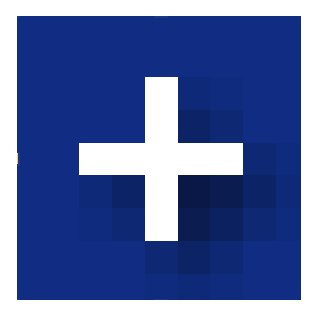
\includegraphics[scale=0.05]{blueicon.eps}
\end{multicols*}
\end{document}

% Page format source: Dave Richeson (divisbyzero.com), Dickinson College% 

% summarised by cos
